\documentclass{article}

\usepackage[margin=1in]{geometry}

\usepackage{lmodern}
\usepackage{amsmath}
\usepackage{amssymb}
\usepackage{upgreek}
\usepackage{pgfplots}
\usepackage[normalem]{ulem}

\pgfplotsset{width=7cm,compat=1.8}
\usetikzlibrary{decorations.markings}


\begin{document}

\section{Curvas Parametrizadas}
De modo geral, podemos descrever uma curva plana por uma \uline{parametriza\c{c}\~ao}:
\[ \vec{r}(t) = (x(t), y(t)) \qquad \text{onde $x(t)$ e $y(t)$ s\~ao fun\c{c}\~oes da vari\'avel $t$.} \]
Exemplo: \\[-5pt]

$y = 2x \quad \rightarrow \quad \vec{r}(t) = (t, 2t)$

\subsection{Vetor Tangente}
O vetor \uline{tangente} \`a curva $\vec{r}(t) = (x(t),\, y(t))$ em um ponto $(x(t_\uplambda),\, y(t_\uplambda))$ \'e:
\[ \vec{v}(t_\uplambda) = \vec{x}\,'(t_\uplambda)\vec{\dot{\imath}} \> + \> \vec{y}\,'(t_\uplambda)\vec{\dot{\jmath}} \]
Denota-se $\vec{r}\,'(t_\uplambda)$. \\[5pt]
Exemplo:

Vetor tangente \`a curva $\vec{r}(t) = (t,\, 2t)$ no ponto $(3, 6)$:
\begin{gather*}
  (3, 6) \>\Rightarrow\> t_\uplambda = 3 \\[5pt]
  \vec{x}\,'(t) = 1 \\
  \vec{y}\,'(t) = 2 \\
  \therefore \\
  \vec{v}\,'(3) = \vec{\dot{\imath}} + 2\vec{\dot{\jmath}}
\end{gather*}
O respectivo vale para curvas no espa\c{c}o.

\subsection{Gr\'aficos}

\begin{tabular}{cc}
  $\vec{r}(t) = (\cos t, 0, \sin t)$ & $\vec{r}(t) = (\cos t, \sin t, t)$ \\[5pt]
  \vtop{\null\hbox{
    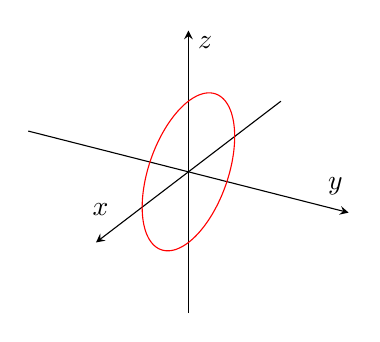
\begin{tikzpicture}
      \begin{axis}[
          view       = {120}{30},
          axis lines = middle,
          xlabel     = $x$,
          ylabel     = $y$,
          zlabel     = $z$,
          zmax       = 2,
          zmin       = -2,
          xmax       = 2,
          xmin       = -2,
          height     = 8cm,
          width      = 8cm,
          xtick      = \empty,
          ytick      = \empty,
          ztick      = \empty
        ]
        \addplot3+ [
          domain    = 0:2*pi,
          samples   = 400,
          samples y = 0,
          mark      = none,
          red,
        ]
        ( {cos(deg(x))}, {0}, {sin(deg(x))} );
      \end{axis}
    \end{tikzpicture}
  }}
  &
  \qquad\vtop{\null\hbox{
    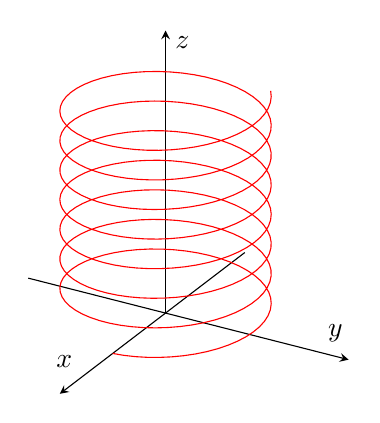
\begin{tikzpicture}
      \begin{axis}[
          view       = {120}{30},
          axis lines = middle,
          xlabel     = $x$,
          ylabel     = $y$,
          zlabel     = $z$,
          zmax       = 60,
          xmax       = 2,
          xmin       = -1.5,
          ymax       = 2,
          ymin       = -1.5,
          height     = 8cm,
          width      = 8cm,
          xtick      = \empty,
          ytick      = \empty,
          ztick      = \empty
        ]
        \addplot3+ [
          domain     = 0:14.7*pi,
          samples    = 400,
          samples y  = 0,
          mark       = none,
          red,
        ]
        ( {cos(deg(x))},{sin(deg(x))},{x});
      \end{axis}
    \end{tikzpicture}
  }}
\end{tabular}

\end{document}
